\chapter{Presentations \& Posters}
\label{ch:visual}

This chapter covers two doctypes for visual communication:
\texttt{presentation} and \texttt{poster}.  Both use sans-serif fonts and
full colour mode, but differ significantly in page size and layout
strategy.

\section{Presentations}
\label{sec:presentation}

The \texttt{presentation} doctype creates slide decks using KOMA-Script
rather than \texttt{beamer}.  It loads
\texttt{lib/layout/omnilatex-presentation.sty}, which provides frame
environments, block environments, progress bars, and section dividers
built with TikZ and tcolorbox.

\subsection{Page Dimensions}

The doctype sets a 16:10 aspect ratio with
\texttt{paperwidth=254mm} and \texttt{paperheight=190.5mm}, applied at
\texttt{\textbackslash AtBeginDocument} via
\texttt{\textbackslash recalctypearea}.  The font size is 14\,pt with
single line spacing.

\subsection{Frame Environments}

Two frame environments are available:

\begin{itemize}
    \item \texttt{presentationframe} -- The primary frame.  Each instance
          triggers a page break, increments the frame counter, renders the
          header and footer, and draws the progress bar before the next
          page break.
    \item \texttt{slideframe} -- A backward-compatible alias that wraps
          \texttt{presentationframe} with identical behaviour.
\end{itemize}

\begin{minted}{latex}
\documentclass[doctype=presentation]{../../omnilatex}
\title{Introduction to OmniLaTeX}
\author{Jane Doe}
\date{2025-11-01}
\begin{document}
\maketitle
\begin{presentationframe}
    \slidetitle{Overview}
    OmniLaTeX is a universal document template.
\end{presentationframe}
\end{document}
\end{minted}

\subsection{Section Dividers}

The \texttt{\textbackslash presentationSection\{title\}} command creates a
full-width coloured section divider.  It fills the upper half of the page
with the university primary colour, centres the section title in large
white bold text, and includes the frame counter and progress bar.

\subsection{Slide Titles}

The \texttt{\textbackslash slidetitle\{...\}} command renders a centred,
coloured title with a decorative rule underneath:

\begin{minted}{latex}
\slidetitle{Key Results}
The experiment confirmed the hypothesis with $p < 0.01$.
\end{minted}

The title is set in \texttt{\textbackslash LARGE\textbackslash bfseries}
in the university primary colour, followed by a 0.6\textbackslash textwidth
rule at 40\% opacity.

\subsection{Multi-Column Layouts}

Two-column slides use the \texttt{presentationcolumns} environment with
\texttt{\textbackslash presentationcolumn\{width\}} commands:

\begin{minted}{latex}
\begin{presentationframe}
    \slidetitle{Comparison}
    \begin{presentationcolumns}
        \presentationcolumn{0.48}
            Left column content.
        \end{column}
        \presentationcolumn{0.48}
            Right column content.
    \end{column}
    \end{presentationcolumns}
\end{presentationframe}
\end{minted}

Note that \texttt{presentationcolumn} opens a \texttt{column} environment
but does not close it; you must end each column with
\texttt{\textbackslash end\{column\}} explicitly.

\subsection{Block Environments}

Five tcolorbox-based block types are provided, each with a coloured left
border and optional title:

\begin{table}[htbp]
    \centering
    \caption{Presentation block environments}
    \label{tab:presentation-blocks}
    \begin{tabular}{@{} l l l @{}}
        \toprule
        \textbf{Environment} & \textbf{Border colour} & \textbf{Background} \\
        \midrule
        \texttt{presentationblock} & University primary & White \\
        \texttt{alertblock}        & Red               & Red!5 \\
        \texttt{exampleblock}      & Green             & Green!5 \\
        \texttt{noteblock}         & Blue              & Blue!5 \\
        \texttt{definitionblock}   & Orange            & Orange!5 \\
        \bottomrule
    \end{tabular}
\end{table}

All blocks accept an optional first argument for additional tcolorbox
options and a mandatory second argument for the title:

\begin{minted}{latex}
\begin{alertblock}{Warning}
    This approach is deprecated.
\end{alertblock}
\begin{definitionblock}{Definition}
    A \emph{group} is a set with an associative binary operation.
\end{definitionblock}
\end{minted}

\subsection{Progress Bar}

A thin progress bar is drawn at the bottom of each slide using TikZ.  It
fills proportionally based on the ratio of the current frame counter to
the total frame count.  The total is computed by calling
\texttt{\textbackslash presentationcountframes} after all frames are
defined.

\subsection{Navigation and Progress Toggles}

\begin{table}[htbp]
    \centering
    \caption{Presentation toggle commands}
    \label{tab:presentation-toggles}
    \begin{tabular}{@{} l l p{5cm} @{}}
        \toprule
        \textbf{Command} & \textbf{Default} & \textbf{Effect} \\
        \midrule
        \texttt{\textbackslash presentationnavsymbolson}  & Off & Show navigation symbols \\
        \texttt{\textbackslash presentationnavsymbolsoff} & Off & Hide navigation symbols \\
        \texttt{\textbackslash presentationprogresson}    & On  & Show progress bar \\
        \texttt{\textbackslash presentationprogressoff}   & On  & Hide progress bar \\
        \bottomrule
    \end{tabular}
\end{table}

Navigation symbols are off by default for clean slides.  The progress bar
is on by default.

\subsection{Frame Counter}

Two counters, \texttt{framecounter} and \texttt{totalframes}, track slide
progression.  The footer displays ``\textit{n\,/\,N}'' in the bottom-right
corner.  Call \texttt{\textbackslash presentationcountframes} at the end
of the document body to set the total.

\section{Posters}
\label{sec:poster}

The \texttt{poster} doctype creates A1 landscape conference posters
(841\,mm $\times$ 594\,mm) with a 20\,pt sans-serif font, \texttt{DIV=20}
layout, and \texttt{paper=a1} base size.  Content is arranged using the
\texttt{multicol} package.

\subsection{Poster Blocks}

Two tcolorbox environments provide titled and untitled content containers:

\begin{itemize}
    \item \texttt{posterblock[title]} -- A titled block with white
          background, dark frame (\texttt{black!70}), 1.5\,pt box rule,
          3\,mm rounded corners, and 8\,mm inner padding.  The title is
          rendered in \texttt{\textbackslash bfseries\textbackslash Large}
          with white text on the frame.
    \item \texttt{posterblocknotitle} -- The same styling without a title
          bar, useful for embedding figures or TikZ diagrams inside a
          titled block.
\end{itemize}

\subsection{Layout Helpers}

\begin{itemize}
    \item \texttt{\textbackslash posterwidth} -- A length set to
          \texttt{0.9\textbackslash textwidth} for consistent block widths.
    \item \texttt{\textbackslash columnbreak} -- Standard
          \texttt{multicol} column break for multi-column poster layouts.
\end{itemize}

\subsection{Example: OmniLaTeX Poster}

The example at \texttt{examples/poster/main.tex} demonstrates a
three-column poster with TikZ graphics:

\begin{minted}{latex}
\documentclass[doctype=poster, institution=none]{../../omnilatex}
\title{OmniLaTeX: A Universal Document Template}
\author{Jane Doe, John Smith}
\date{International Conference on Document Engineering, 2026}
\begin{document}
\maketitle
\begin{multicols}{3}
    \begin{posterblock}[Introduction]
        OmniLaTeX is a modular, universal \LaTeX{} template\ldots
    \end{posterblock}
    \begin{posterblock}[Results]
        \begin{posterblocknotitle}
            \centering
            % pgfplots accuracy chart
            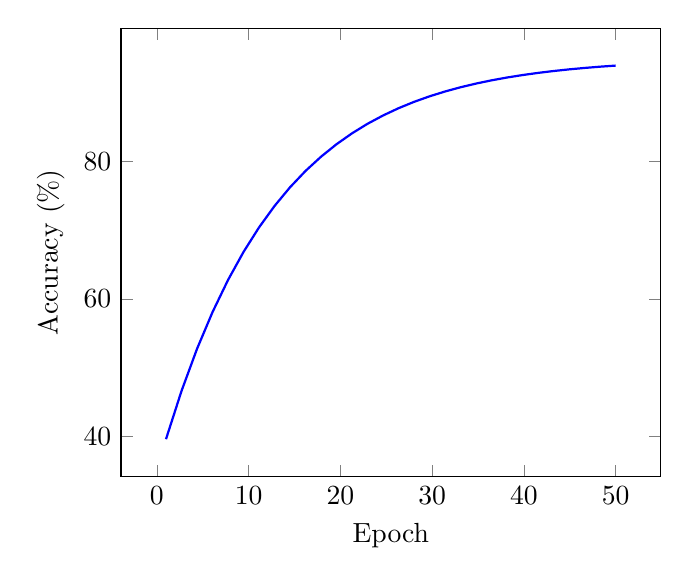
\begin{tikzpicture}
                \begin{axis}[xlabel={Epoch}, ylabel={Accuracy (\%)}]
                    \addplot[blue, thick, domain=1:50, samples=30]
                        {95 - 60*exp(-0.08*x)};
                \end{axis}
            \end{tikzpicture}
        \end{posterblocknotitle}
    \end{posterblock}
    \columnbreak
    \begin{posterblock}[Architecture Overview]
        \begin{posterblocknotitle}
            \centering
            % TikZ system architecture diagram
            \begin{tikzpicture}[
                box/.style={draw, thick, rounded corners,
                    minimum height=8mm, fill=blue!10},
                arr/.style={->, thick, >=stealth},
            ]
                \node[box] (user) {User};
                \node[box, below=of user] (api) {API Layer};
                \node[box, below left=of api] (db) {Database};
                \node[box, below right=of api] (cache) {Cache};
                \draw[arr] (user) -- (api);
                \draw[arr] (api) -- (db);
                \draw[arr] (api) -- (cache);
            \end{tikzpicture}
        \end{posterblocknotitle}
    \end{posterblock}
\end{multicols}
\end{document}
\end{minted}

The title is rendered in 60\,pt bold at the top of the poster, followed by
the author list in \texttt{\textbackslash LARGE} and the date in
\texttt{\textbackslash Large}.  No headers or footers are drawn
(\texttt{pagestyle=empty}).
